\chapter{Conclusiones y trabajo futuro}

	En este trabajo se había planteado como objetivo general el estudio de diferentes técnicas de \gls{nlp}, visión, e inteligencia artificial, con el fin de investigar la posibilidad de automatizar un proceso de valoración de puntos de interés en el mundo real. Esto implicaba tareas con objetivos específicos, como el reconocimiento de objetos en imágenes, y de textos asociados, surgiendo la necesidad de investigar diferentes aproximaciones para resolver estos tipos de problemas, y encontrar la más adecuada. \\
	
	La primera tarea abordada fue la clasificación de imágenes en un conjunto cerrado de clases. Para ello, se decidió utilizar una de las herramientas más populares en problemas de visión artificial que implican tareas como la clasificación o detección de objetos: las redes neuronales convolucionales. Inicialmente, se intentó realizar un entrenamiento desde cero de una \gls{cnn}, lo que resultó en un claro caso de sobreajuste, pues los valores de la función de pérdida sobre el conjunto de validación se disparaban, mientras que los de la función de pérdida sobre el conjunto de entrenamiento tendían a cero. De aquí se obtuvo la conclusión de que se disponía de un número muy reducido de datos de entrenamiento para la cantidad de parámetros a optimizar. A pesar de aplicar técnicas como el aumento de datos, variando parámetros de la imagen como la rotación o el zoom, tampoco se obtuvieron resultados positivos debidos a la insuficiencia datos y persistir el problema del sobreajuste. \\
	
	Ante esta situación, se decidió aplicar la técnica conocida como transfer learning, basada en tomar parámetros de un modelo ya entrenado para un propósito general, de manera que durante el entrenamiento, el resto de parámetros se centren en la tarea específica. En concreto, se tomaron las capas convolucionales del modelo MobileNet de Google, para después añadir capas densas que lograran la clasificación. Gracias a esta técnica, se consiguió eliminar el sobreajuste y clasificar las imágenes en cuatro clases distintas de manera exitosa, obteniendo métricas como un $F_1-$score de $0.97$ o un AuC de $0.99$ sobre un conjunto de imágenes no vistas anteriormente por el modelo. \\
	
	Habiendo conseguido clasificar las imágenes en las cuatro clases originales, se presentó la problemática de poder detectar si una imagen no pertenecía a ninguna de estas. Para ello se plantearon dos soluciones basadas en la anterior. La primera de ellas consistía en añadir una nueva clase a la arquitectura, mientras que la segunda estaba formada por dos \gls{cnn}: una de ellas era capaz de distinguir si una imagen pertenecía a alguna de las clases originales o no, mientras que la otra era capaz de distinguir entre las clases originales. Con el cálculo de probabilidades condicionadas era posible calcular a cuál de las cinco clases (las cuatro originales y una de desconocidos) pertenecía la imagen. Con ambas arquitecturas se obtuvieron resultados muy similares, por lo que se concluyó que era preferible utilizar la primera de ellas, siendo menor el tiempo de cálculo de las predicciones al ser más simple. \\
	
	En este punto se había demostrado que era posible lograr la clasificación de imágenes de un conjunto abierto o cerrado de clases mediante redes convolucionales, pero se presentaban una serie de problemáticas. Si en el futuro se deseaba añadir nuevas clases a las originales, se necesitaba modificar el conjunto de datos, la arquitectura del modelo y reentrenarlo. Además, con la aproximación de \gls{cnn} no se había resulto el problema de trabajar con textos asociados a las imágenes. Tras varias investigaciones surge la idea de trabajar con un tipo de modelos que están a la orden del día, los transformers, específicamente los multimodales, que combinándolos con técnicas de clasificación no supervisada podían solucionar los problemas planteados. \\
	
	Con motivo de añadir un componente de cloud al trabajo, se decidió utilizar un transformer multimodal que es parte de Vertex (\gls{gcp}). Con ayuda de este, se generaron los embeddings de cada imagen, para posteriormente utilizar un algoritmo de clasificación no supervisada como $k-$means o \gls{cja}. Aprovechando que se conocían las clases originales, se utilizaron algunas métricas que proporcionaron valores adecuados, como un ARI de $0.95$ o una $V-$measure de $0.95$. Mediante métricas como el coeficiente de silueta, no se obtuvieron valores óptimos en cuanto a la separación entre clusters, pero las anteriores verificaban la corrección del procedimiento. Gracias a este método, no hacía falta modificar el modelo en caso de desear variar el número de clases, tan solo se debía volver a lanzar el clustering. Además, tampoco era necesario conocer el número de clases, pues mediante el método del codo se podía calcular el óptimo. \\
	
	Con esta arquitectura compuesta por un transformer multimodal y un algoritmo de clasificación no supervisada, se concluyó que era mucho más flexible a cambios futuros en comparación a una basada en \gls{cnn}. Además, permitía resolver el problema de trabajar con textos asociados a las imágenes. La multimodalidad del transformer, permitía generar embeddings de textos en un mismo espacio que los de las imágenes, posibilitando la búsqueda de imágenes mediante descripciones, y la selección del texto que mejor describía una imagen. En general, con ayuda del transformer se consiguió extraer de las imágenes detalles más precisos, textos, e incluso agruparlas por conceptos más abstractos. \\
	
	En cuanto a la clasificación de imágenes, se puede afirmar que, independientemente de las tareas relacionadas con texto u otras modalidades de información, la arquitectura formada por un transformer codificador y un algoritmo de clasificación no supervisada es preferible a una basada en \gls{cnn}. Esta combinación ofrece resultados más precisos y es más flexible ante cambios futuros en el dominio del problema, sin la necesidad de reservar datos de entrenamiento. Para finalizar, se propone como trabajo futuro la automatización de las dos tareas con las que se completaría la automatización del proceso de valoración, pues lo relativo a detección de objetos y textos se ha logrado durante este trabajo. \\
	
	La primera de ellas sería detectar los elementos duplicados, es decir, imágenes del mismo objeto en el mismo lugar con diferentes perspectivas. La segunda de ellas sería la verificación de la ubicación proporcionada, por ejemplo  con ayuda de Street View, verificar si el objeto aparece, si el entorno es similar, etc. Para abordar la primera de ellas, se sugiere comenzar utilizando una técnica similar a la empleada para la búsqueda semántica o selección de descripciones. Se puede calcular el coseno del ángulo formado por el embedding de la imagen propuesta y el de cada una de las candidatas a duplicados, tratando de observar los valores de estos. Para el caso de la \Cref{fig:duplicados} se obtienen los valores de $0.89, 0.75, 0.44$, y $0.49$, notándose un valor mayor para la misma imagen tomada desde otra perspectiva, pudiendo ser este el punto de partida de una futura investigación. La segunda de las tareas es bastante más compleja, lo que requeriría el estudio de técnicas más avanzadas de visión artificial, aunque una posible ayuda podría ser recuperar la ubicación de la imagen mediante alguna herramienta como ExifTool, siempre que el usuario no hubiera desactivado los metadatos, para poder calcular la distancia entre las coordenadas. 
	
	\begin{figure}[!h]
		\centering
		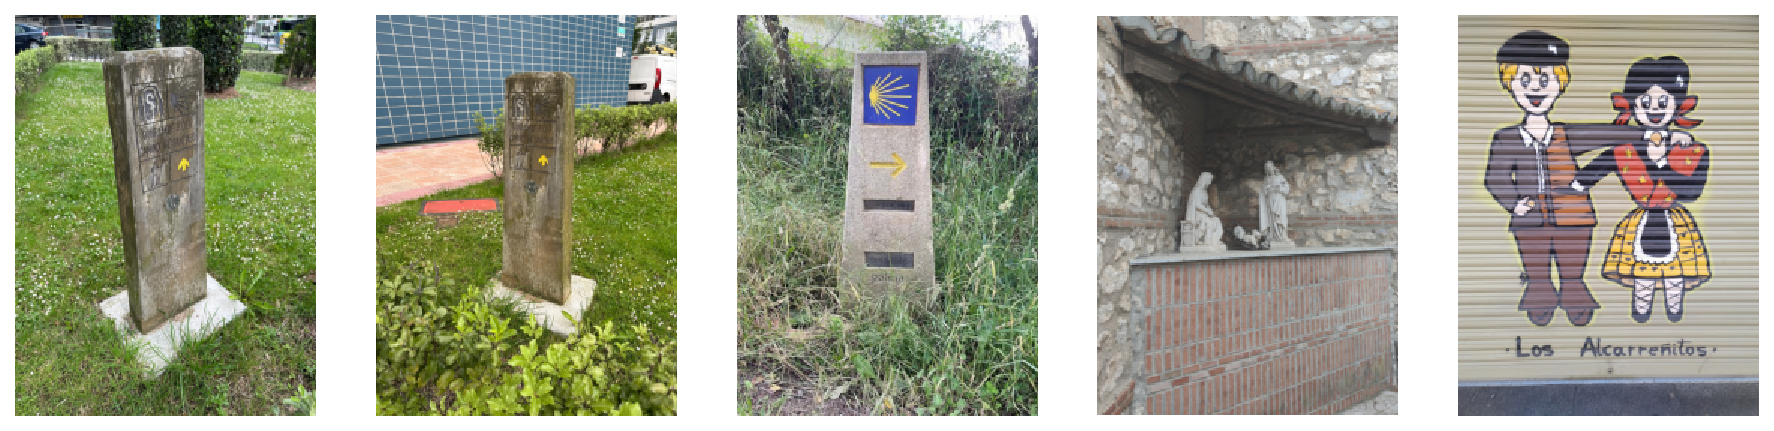
\includegraphics[width = .85\textwidth]{duplicados}
		\caption{Imágenes entre las que detectar duplicados}
		\label{fig:duplicados}
	\end{figure}